\documentclass[../../main.tex]{subfiles}

\begin{document}
Como mencionamos en el Capítulo \ref{chap:problema}, los experimentos fueron realizados con
datos generados sintéticamente, diseñados para imitar situaciones reales. Para comprender
cómo se construyeron estos datos, recordemos que nuestro objetivo es identificar
unidades pertenecientes al grupo de control en escenarios donde la asignación de
individuos (o su inscripción) al tratamiento tiene las siguientes características:
\begin{itemize}[itemsep=0.05cm]
    \item Es no aleatoria.
    \item Es secuencial, es decir que hay cohortes.
    \item Es potencialmente dependendiente de resultados pasados.
\end{itemize}

Dicho esto, la síntesis de los datos involucra la creación de una serie de tiempo
univariada para cada individuo o unidad, que incorpora componentes autorregresivos\footnote{Un
\textbf{proceso autorregresivo de orden uno}, abreviado como \textbf{AR(1)} es un modelo
de series de tiempo en donde el valor actual de la serie depende linealmente de su valor
más reciente más una perturbación impredecible \cite{intro-econometria-wooldridge}. La
fórmula de un AR(1) es la siguiente:
\[
    y_t = \rho \times y_{t-1} + e_t
\]
donde a \(\rho\) se lo denomina coeficiente autorregresivo y \(e_t\) para \(t=0,1,...,T\)
es una secuencia de valores independiente e idénticamente distribuidos con media cero y
varianza \(\sigma_e^2\). Para más información, se puede consultar el Capítulo 11.1 de
\cite{intro-econometria-wooldridge}.}, efectos fijos y efectos temporales\footnote{En el
modelado de series de tiempo, una forma de capturar los efectos no observables que
influyen en la variable dependiente y son constantes en el tiempo consiste en incorporar
un factor denominado \textbf{efecto fijo}, el cual permanece invariante a lo largo de
todos los pasos de tiempo. Para una explicación más detallada, se puede consultar el
Capítulo 13.3 de \cite{intro-econometria-wooldridge}. Similarmente, los efectos no
observables que sí cambian con el tiempo pero que afectan a todos los individos por igual
se conocen como \textbf{efectos temporales}.}, resultando así en un conjunto de datos
de panel. Distinguimos entre tres tipos de individuos:

\begin{itemize}[itemsep=0.1cm]
    \item \textbf{Individuos tratados}: son aquellos que han recibido el tratamiento en
    algún período, es decir que forman parte de alguna de las cohortes.
    \item \textbf{Individuos de control}: son aquellos que en los datos sintéticos,
    sabemos que forman parte del grupo de control para una determinada cohorte de
    tratados. Los llamaremos ``controles''.
    \item \textbf{Individuos ``NiNi''} (``Ni tratados Ni controles''): son aquellas
    unidades que no han sido tratadas y que en los datos sintéticos, sabemos que no forman
    parte del grupo de control para ninguna de las cohortes.
\end{itemize}

Para los tratados y los controles, agregamos una característica extra además de la serie
de tiempo, a la que llamamos ``\textit{inicio de programa} o \textit{tratamiento}''. Para
los primeros, este representa el momento en que un individuo recibió el tratamiento; y
para cada unidad de control, representa el momento en que se aplicó el programa a los
individuos tratados para los cuales efectivamente sirve como control. Si por ejemplo para
un individuo tratado consideramos 20 períodos de tiempo antes del tratamiento, esto quiere
decir que su inicio de programa corresponde el período 21.

Además, al estar en el marco del aprendizaje supervisado, también incluimos la etiqueta
que le corresponde a cada individuo: ``1'' para tratados y controles, y ``0'' para los
NiNi. La razón por la cual tratados y controles comparten la misma etiqueta es que
buscamos que los modelos aprendan durante su entrenamiento los patrones que tienen los
tratados para luego poder clasificar como 1 a aquellos que se les asemejen. Estos serán
justamente los que identifique como potenciales individuos de control.

La motivación detrás de esta construcción artificial es forzar que tanto tratados como
controles compartan una determinada dinámica en su comportamiento temporal, mientras que
los NiNi no. Cabe aclarar que la presencia de la dinámica exacta que modelamos constituye
una hipótesis que en la práctica puede resultar difícil de verificar; y nuestro interés
radica en evaluar si al simularla, los algoritmos son capaces de capturar tales patrones.

Como mencionamos anteriormente, para cada individuo \(i\) generamos una serie de tiempo
univariada \(y_i\) de una longitud \(L\). La fórmula que utilizamos para simular cada
valor \(y_{i,t}\) de las series, con \(t = 0, 1, ..., L\) indicando el período generado,
fue la siguiente:
\begin{align}
    y_{i,0} &= \mu + u_0  \ \sigma \\
    y_{i,t} &= \phi \ y_{i,t-1} + (1 - \phi) \ \mu +  u_t \ \sigma \qquad (t \ge 1)
\end{align}
donde:
\[
    \mu = \mu_{EF} + EF_i + \mu_{ET}
\]
es una constante que depende del individuo \(i\) y:
\begin{itemize}[itemsep=0.1cm]
    \item \(\mu_{EF}\) representa la media de los efectos fijos para todos los individuos
    de un mismo grupo. Denotamos con \(\mu_{{EF}_T}\), \(\mu_{{EF}_C}\) y
    \(\mu_{{EF}_{NiNi}}\) la media de los efectos fijos para tratados, controles y NiNi
    respectivamente. En todos nuestros experiementos, tomamos \(\mu_{{EF}_T} =
    \mu_{{EF}_C} = 10\), y el que sí variamos es \(\mu_{{EF}_{NiNi}}\).
    \item \(\mu_{ET}\) representa la media de los efectos temporales en todos los pasos
    de la serie y es la misma para todos los grupos.
    \item \(EF_i\) representa el efecto fijo del individuo \(i\), constante en todos
    los pasos de tiempo.
    \item \(\phi\) es el componente autorregresivo asociado a la variable generada para
    todos los individuos de un mismo grupo. En nuestros experimentos, usamos \(\phi = 0.9\)
    para todos los grupos.
    \item \(u_t\) es un valor aleatorio proveniente de una distribución normal estándar
    (se genera uno en cada paso de tiempo).
    \item \(\sigma\) es la desviación estándar del término de ruido de las series,
    y es la misma para todos los grupos. En este trabajo, tomamos \(\sigma=5\).
\end{itemize}

Generamos diversos escenarios, todos con 3 cohortes, que se diferencian entre sí por
determinados aspectos:
\begin{enumerate}[itemsep=0.05cm, label=\textbf{\arabic*.}]
    \item La longitud de las series de tiempo generadas, que denotamos con \(L\). Esta
    representa la cantidad de períodos observados para cada individuo \textbf{previos al inicio
    del tratamiento}.
    \item La cantidad de períodos previos al inicio del tratamiento en los que se observa
    un comportamiento específico en tratados y controles. A estos períodos, como
    mencionamos previamente, los llamamos ``\textbf{períodos de dependencia} (temporal)'',
    y son siempre los últimos de los períodos pre-tratamiento. Denotamos la cantidad de
    períodos de dependencia con \(n_{pd}\), y en nuestros escenarios, se va a cumplir
    siempre que \(0 \le n_{pd} < L\).
    \item En los períodos de dependencia, modelos un comportamiento al que llamamos
    ``\textbf{decreciente con ruido}'': en dichos períodos, forzamos a que cada nuevo
    valor generado sea estrictamente menor al anterior, salvo en una cantidad \(m\) de
    ocasiones en donde permitimos que sea mayor, es decir que haya ``subidas'' o
    incrmentos. Este \(m\) también varía entre escenarios. Consideramos que esta tendencia
    es representativa de fenómenos reales, y que puede influir en la decisión que los
    individudos reciban un tratamiento o participen de un programa.
    \item La media de los efectos temporales para los indiviudos NiNi. Puntualmente,
    reducir este valor a la hora de generar los datos provoca que la media de la variable
    dependiente en los NiNi en cada uno de los períodos esté por debajo de la de tratados
    y controles\footnote{Este efecto se verá con mayor claridad en el
    \hyperref[sec:exp4]{Experimento 4} del Capítulo de
    \hyperref[chap:resultados]{Resultados}.}.
\end{enumerate}
Para cada escenario, generamos 100 simulaciones para poder garantizar que los resultados
obtenidos sean estadísticamente significativos.

A modo de ejemplo, la Figura \ref{fig:treated_series_example} muestra el gráfico de 15
series de tiempo generadas para individuos tratados con \(L=45\), \(n_{pd}=20\) y \(m=6\).
Como tenemos 3 cohortes y de cada indivudo estamos tomando los 45 períodos antes que cada
uno haya recibido el tratamiento (independientemente de la cohorte a la que pertenezcan),
los inicios de programa, aunque no se visualizan explícitamente, son 46, 47 y 48 (uno para
cada cohorte).

\begin{figure}[ht]
    \centering
    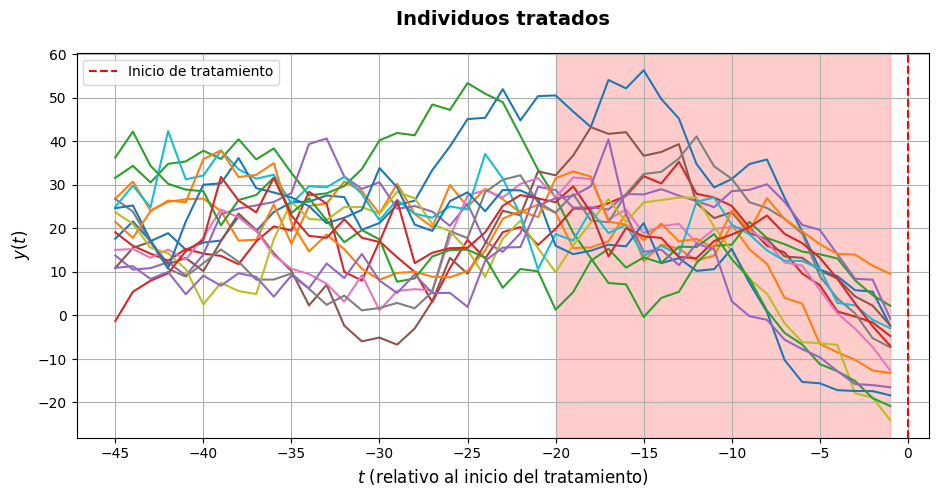
\includegraphics[width=0.8\textwidth]{figs/tratados_exp1_sim13.png}
    \caption{Gráfico de 15 series de tiempo generadas para individuos tratados con
    \(L=45\), \(n_{pd}=20\), y \(m=6\). Los tratados están divididos en cohortes, cada una
    de las cuales tiene su correspondiente inicio de programa, por lo que en el eje \(x\)
    se encuentra el período relativo al inicio de programa de cada individuo (por ejemplo,
    -5 indica el quinto período antes que una unidad reciba el tratamiento,
    independientemente de cuándo lo recibió). El eje \(y\) representa el valor de la
    variable en cada período. La línea vertical punteada de color rojo indica el inicio de
    tratamiento de cada individuo, y los períodos con fondo rojo son los períodos de
    dependencia.}
    \label{fig:treated_series_example}
\end{figure}

En todos los escenarios y simulaciones, la distribución de individuos fue la siguiente:
\begin{itemize}[noitemsep]
    \item Cantidad de individuos tratados: 1000, divididos en las 3 cohortes (334 en la
    primera y la segunda, y 332 en la restante).
    \item Cantidad de individuos de control: 1000, divididos en las 3 cohortes (334 en la
    primera y la segunda, y 332 en la restante).
    \item Cantidad de individuos NiNi: 3500.
\end{itemize}

En la sección \ref{sec:comparacion}, explicamos cómo a partir de los datos generados,
construimos los conjuntos de entrenamiento y test, y cómo fueron utilizados para obtener
los resultados.

A continuación, describimos las diferentes arquitecturas de redes neuronales que
utilizamos durante los experimentos y los valores particulares que fueron incluidos en la
búsqueda de hiperparámetros.

\end{document}